\section{Episodic Logic (EL)}
\label{sec:el}

Before we define Episodic Logic, we should motivate its use for schemas: why do we use EL instead of more ``battle-hardened'' existing logical formalisms? First-order logic (FOL)---used for planning and knowledge representation by the STRIPS planning system \citep{fikes1972}, GENESIS \citep{mooney90}, and many other classical AI systems---would be a natural first choice: its syntax and semantics are simple and known by academics and practitioners alike. However, FOL is an \textit{extensional} logic by nature, and as such does not allow for modal statements such as ``I know that Gaurav loves Mariel''---the proposition ``Gaurav loves Mariel'' only denotes a truth value, and such a sentence would always be equivalent to ``I know that \texttt{TRUE}'' or ``I know that \texttt{FALSE}'', depending on whether Gaurav loves Mariel or not in that world.\footnote{I like to think that he does.}

Additionally, very important to the notion of schemas is the notion of an \textit{episode}, a.k.a. a situation, a.k.a. an event. Schemas are stereotyped patterns of situations, and so a representation of situations is necessary. FOL has traditionally tackled this with Davidsonian \textit{events} \citep{Davidson1967}, where the event is a first-class domain entity passed as an extra argument to situational predicates. As we'll see below, this approach is actually quite similar to how Episodic Logic handles events, except that Davidsonian event variables can only be passed to positive, atomic predication literals; Episodic Logic's semantics allow arbitrarily complex formulas to hold in certain events.
% This has only been a sketchy outline of a few key differences between FOL and EL; for a more thorough comparison, please refer to \citep{schubert2000episodic}.

\subsection{What is EL?}
EL is a predicate logic whose semantics are intended to model some important aspects of natural language, and of the human thought patterns that give rise to natural language. As its name implies, one of EL's most distinctive features is its use of \textit{episode} variables to denote time-bounded ``temporal'' propositions, such as ``Palutena is sleepy'' or ``I'll go running for an hour''---as well as ``atemporal'' propositions, which necessarily hold true eternally, like ``hydrogen is an element'' or $2+3=5$.

EL naturally supports other aspects of natural language as well. It is an \textit{intensional} logic: a sentence like ``Gaurav loves Mariel'' can represented as not just a truth value, but as a function from possible situations to truth values called a \textit{sentence intension}. Sentence intensions may be transmuted into individuals using \textit{reification} operator \texttt{That}, and predicates may be similarly reified into individuals with the kind-forming operator \texttt{K}\footnote{Or \texttt{Ke} for forming kinds of events, or \texttt{Ka} for forming kinds of actions.}; this allows abstract entities, such as \textit{``the process of writing a dissertation''}, as well as concrete entities, such as \textit{``Lane's dissertation''}, to act as predicate arguments without defining special semantics for higher-order predicates (that is, predicates with predicate arguments).

EL's episodes are associated with EL formulas primarily via the \textit{characterizing} operator \texttt{**}. Intuitively, the EL form of sentence like ``I am writing my dissertation'' \textit{characterizes} an episode \texttt{e}, then \texttt{e} is an ``episode \textit{of}'' me writing my dissertation. This is contrasted with the operator \texttt{*}; while \el{[$\phi$ ** e]} means that \el{e} is an episode \textit{of} \el{$\phi$}, \el{[$\phi$ * e]} only asserts that \el{$\phi$} is \textit{true in} \el{e}. While it is always true that \el{[$\phi$ ** e]} $\implies$ \el{[$\phi$ * e]}, the converse is not necessarily true: the sun setting could be true in an episode \textit{of} me writing my dissertation, but that does not also make it an episode \textit{of} the sun setting.



\subsection{Explanation of an example}
As EL is intended as a representation for natural language, we often make use of primarily lexical predicates, which represent verbs, nouns, adjectives, and other words. The nature of these lexical predicates, and the rough capabilities of EL's semantics to relate them, may be best presented---for our purposes---by the explanation of some illustrative examples. Let's first look at an English sentence and its EL form, and then note its meaning and various features---as well as some features of EL that may not be covered in the example.

%\textbf{English}: \textit{Rivka insisted that she had eaten food.}

%\textbf{EL}: \el{\footnotesize [$\exists$ e1 : [e1 before Now] [|Rivka| insist.v (That ($\exists$ e2 : [e2 before e1] [(|Rivka| eat.v (K food.n)) ** e2])])] ** e1]}

\textbf{English}: \textit{Rivka insisted that she didn't eat chametz.}

\textbf{EL}:  \el{[E1.sk before Now0],
     [[|Rivka| insist.v
       (that
        (some e2 [e2 at-or-before E1.sk]
              [(not [|Rivka| eat.v (K chametz.n)]) ** e2]))]
      ** E1.sk)}



%\subsubsection{Clarifications}
%The EL here might be a bit hard to read, so I'll clarify it a bit with a ``translation'' of it back into English: \textit{``Some time e1 before now is characterized by Rivka insisting that Rivka eating food characterizes some time e2 before e1.''}

\subsubsection{Restricted quantification}
The existential quantifications of \el{e1} and \el{e2}\footnote{E1.sk is a Skolem constant---it has been assigned a name to remove the top-level existential quantification.} illustrate the ``restrictor-matrix'' structure of EL quantification: if \el{x} is a variable, \el{Q} is a quantifier, and $\phi$ and $\psi$ are arbitrary EL formulas, the quantification formula \el{[Q x : $\phi$ $\psi$]} predicates the truth of the ``restrictor'' formula $\phi$ whenever the ``matrix'' formula $\psi$ holds true. When \el{Q} is $\exists$, this is equivalent to the unrestricted quantification \el{[$\exists$ x ($\phi \land \psi$)]}; similarly, when \el{Q} is $\forall$, it is equivalent to \el{[$\forall$ x ($\phi \rightarrow \psi$)]}. The restrictor-matrix form is only necessary for some of EL's nonstandard quantifiers, e.g. \el{Many} and \el{Few}, which cannot be reduced to an unrestricted form.

\subsubsection{Temporal relations}
The temporal relation \el{before} is used to relate the time of \el{E1.sk} to the special time constant \el{Now0}---which represents the time that the speaker is uttering this---and the time of \el{e2} to \el{E1.sk}, and thus also \el{e2} to \el{Now}. Such temporal relations---as well as the tacit temporal relations in their transitive closures---place the episode times within the ontological domain $\mathcal{R}_{4}$, representing spacetime, and connect their trajectories (see Figure~\ref{fig:el_ontology}). More temporal relations exist, special functions \el{start-of(e)} and \el{end-of(e)} allow temporal predications about the instantaneous endpoints of episodes, and disjoint intervals may even form an episode; for more information on the temporal semantics of EL, please refer to \citep{hwang1993}.

\subsubsection{Representing sentences}
``Sentences'' in EL are often verb predications: the heart of this one is the 2-place predicate \el{insist.v}, with \el{|Rivka|} as the first argument, and a \el{That}-reified sentence as the second. This syntax is just a ``pretty'' version that reflects the subject-verb-object nature of the English language; semantically, it would be more honest to write the predication out with the arguments all postfixed, but nobody wants to see that.

\subsubsection{Reification and \textit{kind}-forming}
The kind-forming operator \el{K} is used here because \el{chametz.n} is a one-place predicate that determines whether its argument is is chametz\footnote{Food containing leaven; prohibited during Pesach, a.k.a. Passover.}. So, because we don't know the specific chametz individual, we choose to make a statement about her eating a \text{kind of chametz}, which we accomplish by \textit{reifying} the \el{chametz.n} predicate, rather than \textit{Skolemizing} a variable (i.e. assigning it a concrete name, to bypass existential quantification) and attaching the predicate to it (i.e. assigning it a name).
\footnote{Well, it actually provides a function from possible situations to whether its argument is food in each of those situations, but I've omitted this detail for clarity \textit{supra}, preferring instead this footnote: an intentional extensional intension extension.}
In order to use a predicate as an argument to another predicate, we must first reify it as an individual.

We can reify other sorts of things, too. The reified verb phrase \el{(Ka (drink.v (K water.n)))}
\footnote{What's being reified is actually not a well-formed EL predication, assuming \el{drink.v} is a 2-place predicate; the actor argument is missing! What's \textit{actually} being reified here, implicitly using the \el{K} operator, is something like the \textit{lambda abstraction} \el{($\lambda$a (a drink.v (K water.n)))}; however, even that's not quite right, as there are additional complications related to event characterization. For a full discussion of this, see page 7 of \citep{schubert2000episodic}.}
is the \textit{kind of action} of drinking water, and belongs to the class $\mathcal{K}_{A}$ in the EL ontology (see Figure~\ref{fig:el_ontology}). 

The reified sentence \el{(Ke (|Mary| drink.v (K water.n)))} is the \textit{kind of event} where Mary drinks water, and belongs to the ontological class $\mathcal{K}_{E}$. This is semantically distinct from the other reification of this sentence, which uses the \el{That} operator, \el{(That (|Mary| drink.v (K water.n)))}, which is a \textit{proposition}, and thus belongs to the ontological class $\mathcal{P}$. An intuition for their semantic distinction is quite easy to obtain from the names of their operators: ``the kind of event of Mary drinking water'' is obviously different from ``that Mary is drinking water''.

\subsubsection{The \el{**} and \el{*} operators}
\el{**} and \el{*} are \textit{modal} operators: statements like \el{[$\phi$ ** e]} and \el{[$\psi$ * e]} may not, in general, have their formula arguments, $\phi$ and $\psi$, replaced with other formulas that seem to have the same truth value. So, the EL formula \el{((|Andre| sleep.v) * e)} does \textit{not} entail \el{(((|Andre| sleep.v) $\land$ ( (|Fido| bark.v) $\lor$ $\neg$ (|Fido| bark.v) )) * e)}, even though it would seem to have the same truth value; in fact, the entity \el{|Fido|} might not have any role in the episode, and so even tautological statements involving it may have no binary truth value in \el{e}.

\subsubsection{Characterization by a negative}
Unlike Davidsonian events, EL episodes can be characterized by arbitrarily complex EL formulas, including negatives. Here, \el{e2} is an episode of Rivka \textit{not} eating.

\subsection{Discussion}
I'll leave aside any further description of EL's features or formal semantics, as I think the analysis above has demonstrated what I intended it to: that Episodic Logic is an expressive language with rich, event-oriented semantics. In the sections to come, it will become clearer how these semantics naturally support schema-based reasoning. However, it is worth mentioning that EL is not only expressive, but that EL \textit{inference} is \textit{tractable}; it might seem that ``the richer the model, the longer it stalls'', but EPILOG, the main implementation of EL inference, has comparable performance to FOL inference systems on some standard theorem proving tasks \citep{morbini2009evaluation}. Although EPILOG is somewhat slower than state-of-the-art FOL engines on theorem proving tasks, it also provides more powerful inference rules, and can compute certain sorts of inferences whose FOL equivalents would take time to be translated before inference could even begin.

Additionally, EL is much closer to the ``surface form'' of natural English text than FOL, owing to its intensional predicates, flexible quantifiers, and other features. This surface similarity to natural language is quite beneficial for the task of parsing natural language text into EL. EL also has an ``underspecified'' form, which lacks certain features of EL---e.g. quantifier scoping, and the conversion of grammatical information, like tense, into temporal predications about episodes---but still represents the semantic type structure of a sentence. This form is called ``ULF'' (underspecified logical form) \citep{kim2019type}, and it is a practical, intermediate target form for the mass-parsing of text corpora that is still useful for many applications---such as simple schemas. In fact, using ULF for schemas may actually help convert ULF to full EL, by incorporating the knowledge represented by the schemas into the parsing pipeline. We explore the use of ULF, and EL, for schemas in later sections.

\begin{figure}
    % Made with matchcha.io---strong recommendation from me! :)

%\epigraph{\textit{There are more things in heaven and earth, Horatio, Than are dreamt of in your philosophy.}}{---William Shakespeare, \textit{Hamlet}}

\tikzset{every picture/.style={line width=0.75pt}} %set default line width to 0.75pt        

\begin{center}
\scalebox{1.0}{
\makebox[\textwidth][c]{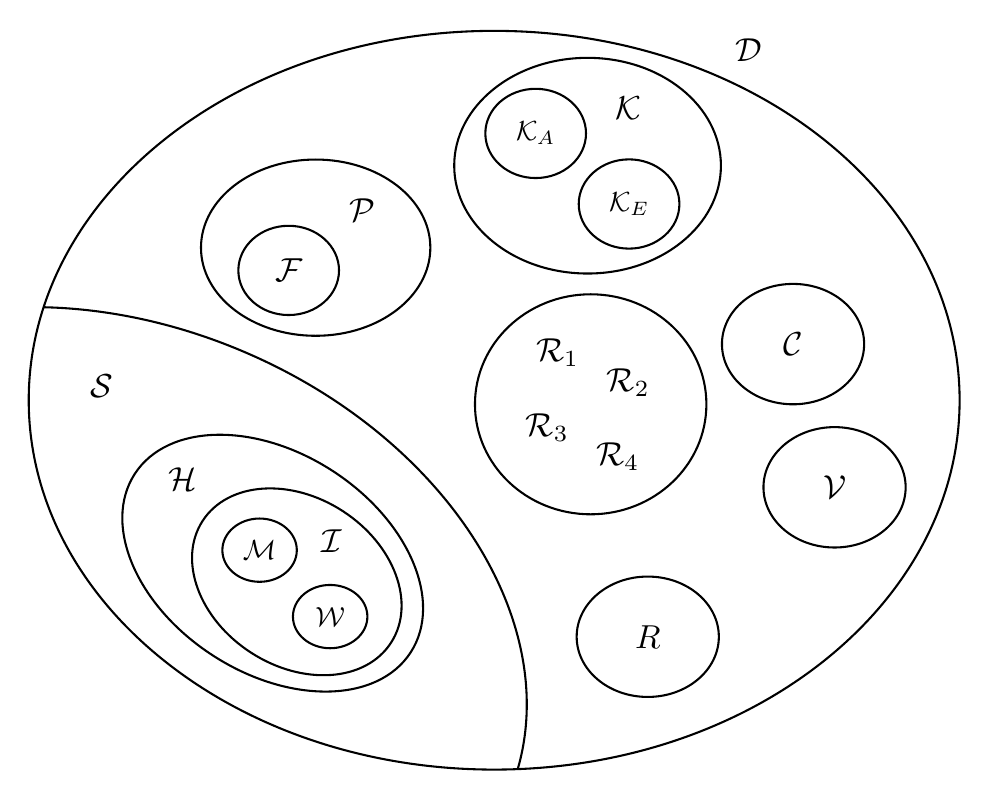
\begin{tikzpicture}[x=0.75pt,y=0.75pt,yscale=-1,xscale=1,scale=1,every node/.style={scale=1}]
%uncomment if require: \path (0,721.921875); %set diagram left start at 0, and has height of 721.921875

%Shape: Ellipse [id:dp9100065238827619] 
\draw   (98,300.96) .. controls (98,202.68) and (198.4,123) .. (322.25,123) .. controls (446.1,123) and (546.5,202.68) .. (546.5,300.96) .. controls (546.5,399.25) and (446.1,478.92) .. (322.25,478.92) .. controls (198.4,478.92) and (98,399.25) .. (98,300.96) -- cycle ;
%Shape: Ellipse [id:dp10388374342633644] 
\draw   (181,227.46) .. controls (181,204.01) and (205.74,185) .. (236.25,185) .. controls (266.76,185) and (291.5,204.01) .. (291.5,227.46) .. controls (291.5,250.91) and (266.76,269.92) .. (236.25,269.92) .. controls (205.74,269.92) and (181,250.91) .. (181,227.46) -- cycle ;
%Shape: Ellipse [id:dp27736097111625835] 
\draw   (199,238.42) .. controls (199,226.55) and (209.86,216.92) .. (223.25,216.92) .. controls (236.64,216.92) and (247.5,226.55) .. (247.5,238.42) .. controls (247.5,250.3) and (236.64,259.92) .. (223.25,259.92) .. controls (209.86,259.92) and (199,250.3) .. (199,238.42) -- cycle ;
%Shape: Ellipse [id:dp7888799168086817] 
\draw   (303,187.96) .. controls (303,159.26) and (331.77,136) .. (367.25,136) .. controls (402.73,136) and (431.5,159.26) .. (431.5,187.96) .. controls (431.5,216.66) and (402.73,239.92) .. (367.25,239.92) .. controls (331.77,239.92) and (303,216.66) .. (303,187.96) -- cycle ;
%Shape: Ellipse [id:dp4804121479534271] 
\draw   (363,206.42) .. controls (363,194.55) and (373.86,184.92) .. (387.25,184.92) .. controls (400.64,184.92) and (411.5,194.55) .. (411.5,206.42) .. controls (411.5,218.3) and (400.64,227.92) .. (387.25,227.92) .. controls (373.86,227.92) and (363,218.3) .. (363,206.42) -- cycle ;
%Shape: Ellipse [id:dp0795716353230258] 
\draw   (318,172.42) .. controls (318,160.55) and (328.86,150.92) .. (342.25,150.92) .. controls (355.64,150.92) and (366.5,160.55) .. (366.5,172.42) .. controls (366.5,184.3) and (355.64,193.92) .. (342.25,193.92) .. controls (328.86,193.92) and (318,184.3) .. (318,172.42) -- cycle ;
%Shape: Ellipse [id:dp12618348576003102] 
\draw   (432,273.92) .. controls (432,257.91) and (447.33,244.92) .. (466.25,244.92) .. controls (485.17,244.92) and (500.5,257.91) .. (500.5,273.92) .. controls (500.5,289.94) and (485.17,302.92) .. (466.25,302.92) .. controls (447.33,302.92) and (432,289.94) .. (432,273.92) -- cycle ;
%Shape: Ellipse [id:dp8799691211755756] 
\draw   (452,342.92) .. controls (452,326.91) and (467.33,313.92) .. (486.25,313.92) .. controls (505.17,313.92) and (520.5,326.91) .. (520.5,342.92) .. controls (520.5,358.94) and (505.17,371.92) .. (486.25,371.92) .. controls (467.33,371.92) and (452,358.94) .. (452,342.92) -- cycle ;
%Shape: Ellipse [id:dp824996442524188] 
\draw   (362,414.92) .. controls (362,398.91) and (377.33,385.92) .. (396.25,385.92) .. controls (415.17,385.92) and (430.5,398.91) .. (430.5,414.92) .. controls (430.5,430.94) and (415.17,443.92) .. (396.25,443.92) .. controls (377.33,443.92) and (362,430.94) .. (362,414.92) -- cycle ;
%Shape: Ellipse [id:dp8272383634329143] 
\draw   (313,302.92) .. controls (313,273.65) and (337.96,249.92) .. (368.75,249.92) .. controls (399.54,249.92) and (424.5,273.65) .. (424.5,302.92) .. controls (424.5,332.19) and (399.54,355.92) .. (368.75,355.92) .. controls (337.96,355.92) and (313,332.19) .. (313,302.92) -- cycle ;
%Shape: Arc [id:dp39537977602891705] 
\draw  [draw opacity=0] (105.32,256.16) .. controls (135.93,256.87) and (168.45,263.64) .. (200.4,277.07) .. controls (297.72,317.98) and (354.69,406) .. (333.59,478.73) -- (143.5,412.42) -- cycle ; \draw   (105.32,256.16) .. controls (135.93,256.87) and (168.45,263.64) .. (200.4,277.07) .. controls (297.72,317.98) and (354.69,406) .. (333.59,478.73) ;
%Shape: Ellipse [id:dp5287011551360823] 
\draw   (149.07,336.49) .. controls (164.96,311.91) and (207.6,311.22) .. (244.32,334.95) .. controls (281.04,358.69) and (297.92,397.86) .. (282.03,422.44) .. controls (266.14,447.02) and (223.49,447.71) .. (186.77,423.97) .. controls (150.06,400.24) and (133.18,361.07) .. (149.07,336.49) -- cycle ;
%Shape: Ellipse [id:dp015166695228427951] 
\draw   (181.78,359.11) .. controls (193.96,340.26) and (224.16,338.12) .. (249.23,354.32) .. controls (274.3,370.53) and (284.75,398.94) .. (272.56,417.79) .. controls (260.38,436.64) and (230.18,438.78) .. (205.11,422.58) .. controls (180.04,406.37) and (169.59,377.96) .. (181.78,359.11) -- cycle ;
%Shape: Ellipse [id:dp4822793325306267] 
\draw   (191.3,373.21) .. controls (191.3,364.79) and (199.33,357.96) .. (209.23,357.96) .. controls (219.14,357.96) and (227.17,364.79) .. (227.17,373.21) .. controls (227.17,381.63) and (219.14,388.45) .. (209.23,388.45) .. controls (199.33,388.45) and (191.3,381.63) .. (191.3,373.21) -- cycle ;
%Shape: Ellipse [id:dp37988107849014874] 
\draw   (225.3,405.21) .. controls (225.3,396.79) and (233.33,389.96) .. (243.23,389.96) .. controls (253.14,389.96) and (261.17,396.79) .. (261.17,405.21) .. controls (261.17,413.63) and (253.14,420.45) .. (243.23,420.45) .. controls (233.33,420.45) and (225.3,413.63) .. (225.3,405.21) -- cycle ;

% Text Node
\draw (133,294) node [scale=1.2]  {$\mathcal{S}$};
% Text Node
\draw (244,369) node [scale=1.2]  {$\mathcal{I}$};
% Text Node
\draw (209.23,373.21) node [scale=1]  {$\mathcal{M}$};
% Text Node
\draw (243.23,405.21) node [scale=1]  {$\mathcal{W}$};
% Text Node
\draw (172.23,339.21) node [scale=1.2]  {$\mathcal{H}$};
% Text Node
\draw (396.25,414.92) node [scale=1.2]  {$\mathbb{R}$};
% Text Node
\draw (352.8,278.27) node [scale=1.2]  {$\mathcal{R}_{1}$};
% Text Node
\draw (386.8,292.27) node [scale=1.2]  {$\mathcal{R}_{2}$};
% Text Node
\draw (347.8,314.27) node [scale=1.2]  {$\mathcal{R}_{3}$};
% Text Node
\draw (381.8,328.27) node [scale=1.2]  {$\mathcal{R}_{4}$};
% Text Node
\draw (386.8,160.27) node [scale=1.2]  {$\mathcal{K}$};
% Text Node
\draw (342.25,172.42) node [scale=1]  {$\mathcal{K}_{A}$};
% Text Node
\draw (387.25,206.42) node [scale=1]  {$\mathcal{K}_{E}$};
% Text Node
\draw (466.25,273.92) node [scale=1.2]  {$\mathcal{C}$};
% Text Node
\draw (486.25,342.92) node [scale=1.2]  {$\mathcal{V}$};
% Text Node
\draw (258.8,209.27) node [scale=1.2]  {$\mathcal{P}$};
% Text Node
\draw (223.25,238.42) node [scale=1.2]  {$\mathcal{F}$};
% Text Node
\draw (444.8,132.27) node [scale=1.2]  {$\mathcal{D}$};


\end{tikzpicture}}}
\end{center}

\small
\makebox[\textwidth][c]{\begin{tabular}{c c l}
   & & \\
   $\mathcal{D}$  & & The full \textit{domain} of EL individuals; the union of all following sets \\
   $\mathcal{S}$  & & Possible situations, a.k.a. \textit{episodes}, forming a join semilattice in any given possible world \\
   $\mathcal{H}$  & & Informationally-maximal episodes, a.k.a. \textit{exhaustive situations} \\
   $\mathcal{I}$  & & Spatially-maximal exhaustive situations, a.k.a. \textit{possible times}, a.k.a intervals \\
   $\mathcal{W}$  & & Spatiotemporally-maximal intervals, a.k.a. \textit{possible worlds} \\
   $\mathcal{M}$  & & Spatially-maximal, temporally-minimal intervals, a.k.a. \textit{moments of time} \\
   $\mathcal{P}$  & & \textit{Propositions} \\
   $\mathcal{F}$  & & Consistent propositions, a.k.a. \textit{possible facts} \\
   $\mathcal{K}$  & & \textit{Kinds of individuals}, whose realizations are ordinary individuals \\
   $\mathcal{K}_{A}$  & & \textit{Kinds of actions}, whose realizations are pairs of ordinary individuals and situations \\
   $\mathcal{K}_{E}$  & & \textit{Kinds of episodes}, whose realizations are situations for which a particular characterization holds \\
   $\mathcal{C}$  & & \textit{Collections} of individuals \\
   $\mathcal{V}$  & & \textit{$n$-tuples} of individuals, $n \geq 2$ \\
   $\mathbb{R}$  & & \textit{The real numbers} \\
   $\mathcal{R}_{1}$  & & \textit{Clock times, a uniformly discretized subset of $\mathbb{R}$}, containing subsets of $\mathbb{R}_{n}$
   %& & Note that $\mathcal{R}_{4}$, which represents space-time regions, contains some unconnected \\
   %& & space-time trajectories; these trajectories describe the time and place of episodes.
\end{tabular}}

    \caption{This represents the EL ontology. I include only some brief definitions of the notable subsets; for more formal detail, please refer to \citep{schubert2000episodic}. \tiny{(I'd like to thank \href{https://www.mathcha.io}{mathcha.io} for making the construction of this TikZ figure so painless with their graphical editor.)}}
    \label{fig:el_ontology}
\end{figure}